\documentclass{beamer}


\usepackage{soul}

% TABLES
\newcommand{\ra}[1]{\renewcommand{\arraystretch}{#1}} % spaces in tables
\usepackage{booktabs}   % Allows the use of \toprule, \midrule and \bottomrule in tables for horizontal lines

% LISTS
% \usepackage{enumitem} % Changes the itemize and enumerate


% PSTRICKS
% \usepackage{pstricks,pst-node,pst-tree} % includes graph additions
% \usepackage{pst-pdf} % Compiles the pictures
% \usepackage{pst-node}
% \usepackage{pst-plot}
% \psset{xunit=1cm,yunit=1cm}


% INCLUDE GRAPHICS
\usepackage{graphicx}


% LOGO POSITION
\usepackage{pgf}
% \usepackage[absolute,overlay]{textpos}


% FONTS
% \usefonttheme{serif}
\usefonttheme[onlymath]{serif} % Standard font for math enviroments
\usepackage[T1]{fontenc}
%\usepackage{inconsolata} % Nice monospaced font



% CODE
\usepackage{listings} % Code block (source code) \begin{lstlisting} 

\lstset{
    language=Python,                        % Code langugage
    commentstyle=\color{gray},              % Comments font
    basicstyle=\small\ttfamily,             % Code font, Examples: \footnotesize, \ttfamily
    keywordstyle=\bfseries\color{blue},
    stringstyle=\color{orange},
    numbers=left,                           % Line nums position
    numberstyle=\tiny,                      % Line-numbers fonts
    stepnumber=1,                           % Step between two line-numbers
    numbersep=5pt,                          % How far are line-numbers from code
    numbers=none,
    frame=single,                             % A frame around the code
    tabsize=4,                              % Default tab size
    captionpos=b,                           % Caption-position = bottom
    breaklines=true,                        % Automatic line breaking?
    breakatwhitespace=false,                % Automatic breaks only at whitespace?
    showspaces=false,                       % Dont make spaces visible
    showstringspaces=false,                 % Dont make spaces visible in strings
    showtabs=false,                         % Dont make tabls visible
    belowskip=8pt,
    morekeywords={range, xrange},
    backgroundcolor=\color{white}
    % emph={[2]root,base}
    % morekeywords={one,two,three,four,five,six,seven,eight,
}



\newcommand{\code}[1]{{\small\ttfamily #1}} % \code{inline code}


% BEAMER COLORS
\definecolor{kugreen}{RGB}{50,93,61}
\setbeamercolor{frametitle}{fg=black}
\setbeamercolor{normal text}{fg=black}
\setbeamercolor{structure}{fg=kugreen}

% BEAMER STYLE
\setbeamertemplate{itemize item}{$\bullet$}
\setbeamersize{text margin left=10pt}
\setbeamersize{text margin right=10pt}
\setbeamersize{sidebar width right=0pt}
\setbeamersize{sidebar width left=0pt}
\setbeamercolor{block title}{fg=white,bg=kugreen}
\setbeamercolor{block body}{fg=black,bg=white!95!black}


% BEAMER HEADLINE
\setbeamertemplate{headline}
{%
    % \vbox{

    % \vspace{2pt}

    % \hspace{10pt}
    % \tiny
    % \rmfamily
    % \expandafter\insertshortauthor
    %     \vspace{1pt}
    % }
}


% BEAMER TITLE
\setbeamertemplate{frametitle}
{
    \color{kugreen}
    \begin{centering}\medskip
        \insertframetitle\par
    \end{centering}
}


% BEAMER FOOTER
\setbeamertemplate{footline}[text line]
{%
    \vbox{%
        \tiny\ttfamily
        \insertvrule{0.5pt}{kugreen}

        \vspace{2pt}

        \strut{
        \rmfamily\itshape
        \expandafter\insertshorttitle
        \expandafter\insertauthor,
        \insertshortinstitute
        }
        \hfill\strut{
        }
        \hfill\strut{
            \insertframenumber\,/\,\inserttotalframenumber
            % 
\includegraphics[width=20pt,natwidth=610,natheight=642]{KUNATLogo.pdf}
        }

        \vspace{1pt}
    }
}

\setbeamertemplate{background}{
    % \hspace{330pt}
\includegraphics[width=25pt,natwidth=610,natheight=642]{KUNATLogo.pdf}
}

% BEAMER Frontpage
\setbeamertemplate{title page}
{

    \begin{beamercolorbox}[center]{beamer color}

        {
            \huge
            \color{kugreen}
            \inserttitle
        }
        \bigskip
        \bigskip

        
\includegraphics[width=2cm]{KUNATLogo}

        \bigskip
        {
            \bf
            \rmfamily
            {\large \insertauthor}
        }

        \smallskip
        {
            \rmfamily
            \footnotesize
            \insertinstitute
        }

        {
            \rmfamily
            \footnotesize
            \insertdate
        }

    \end{beamercolorbox}


    \addtocounter{framenumber}{-1}
}

% Removes the navigation bar
\beamertemplatenavigationsymbolsempty

% CONTENT

\logo{\pgfputat{\pgfxy(-1,-0.435)}{\pgfbox[center,base]{
\includegraphics[width=1.2cm,natwidth=610,natheight=642]{KUNATLogo.pdf}}}}



\title[]{Molecular Statistics, Week 2}
\institute[University of Copenhagen]{Department of Chemistry \\ University of Copenhagen}
\author[Jimmy Charnley Kromann]{Jimmy Charnley Kromann}
\date{2014}

\begin{document}

\frame[plain]{\titlepage}


\begin{frame}[fragile]

    \frametitle{Week 2, Lecture Goals}

    \begin{itemize}
        \item Functions
        \item File read/write
        \item Week 1 problems
        \item Debugging
        \item General program structure
    \end{itemize}

    \bigskip

    Note:
    \begin{itemize}

        \item Play around, and you learn

    \end{itemize}

\end{frame}


\begin{frame}[fragile]

    \frametitle{Functions}

    \begin{align*}
        y(x) = x^2
    \end{align*}

    \bigskip
    \bigskip

\begin{lstlisting}
def square(x):
    y = x**2
    return y

\end{lstlisting}

\begin{lstlisting}
print square(5.0)

\end{lstlisting}



\end{frame}


\begin{frame}[fragile]

    \frametitle{Create a Gaussian function}

    \begin{columns}[t]

        \column{0.4\linewidth}

        \begin{align*}
            g(x) = a \exp \left (-\frac{(x-b)^2}{(2c^2)} \right ) + d
        \end{align*}

        \smallskip

        with the following constants

        \begin{align*}
            a = 1.0\\
            b = 0.0\\
            c = 1.0\\
            d = 0.0
        \end{align*}

        \column{0.4\linewidth}

            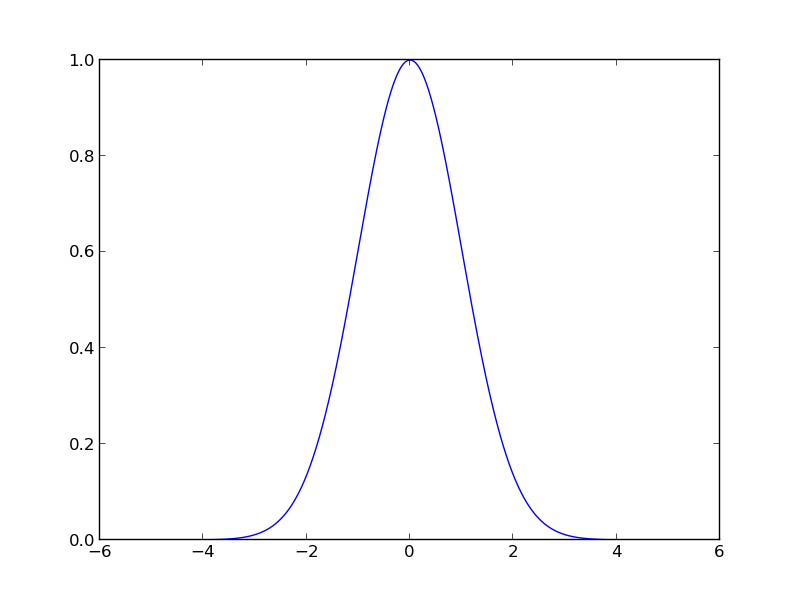
\includegraphics[width=1.0\linewidth]{gaussian.png}

    \end{columns}

\end{frame}


\begin{frame}[fragile]

    \frametitle{Gaussian Function}

\begin{lstlisting}
def gaussian(x):

    a = 1.0
    b = 0.0
    c = 1.0
    d = 0.0

    g = a*np.exp( -(x-b)**2 / (2*c**2) ) + d

    return g

\end{lstlisting}

\begin{lstlisting}
print gaussian(0.0)
\end{lstlisting}

\end{frame}


\begin{frame}[fragile]

    \frametitle{Gaussian Function}

    Multiple parameters

    \bigskip

\begin{lstlisting}
def gaussian(x, a):

    b = 0.0
    c = 1.0
    d = 0.0

    g = a*np.exp( -(x-b)**2 / (2*c**2) ) + d

    return g
\end{lstlisting}

\begin{lstlisting}
print gaussian(0.0, 1.0)
\end{lstlisting}

\end{frame}

\begin{frame}[fragile]

    \frametitle{files}

\begin{lstlisting}
f = open('filename', 'w')
f.write('line text')
\end{lstlisting}

\begin{lstlisting}
f = open('filename', 'r')
for line in file:
    print line
\end{lstlisting}

\end{frame}


\begin{frame}[fragile]

    \frametitle{Bifurcation diagram}

    \begin{equation*}
        x_{n+1} = x_n^2 - r
    \end{equation*}

\end{frame}


\begin{frame}[fragile]

    \frametitle{Week 1 problems}

    What was the hardest part of week 1?\\

    \bigskip

\begin{lstlisting}
pos_x = [random.random() for i in range(n_particles)]

for i in range(n_particles):
    print pos_x[i]

\end{lstlisting}


\end{frame}




\begin{frame}[fragile]

    \frametitle{Debugging}


    \begin{columns}[t]

        \column{0.4\linewidth}

    Typical errors:

    \begin{itemize}
        \item Indentation error
        \item Out of bounds
        \item Object not callable
        \item Invalid syntax
    \end{itemize}

        \column{0.5\linewidth}

        
            
\includegraphics[width=0.8\linewidth]{flip.jpg}

    \end{columns}


\end{frame}



\begin{frame}[fragile]

    \frametitle{Exercise Week 2}

\begin{lstlisting}

import random

...

def initialize_particles(n_particles):
    """ Initialze particles , positions and velocities
    """
    return pos_x , pos_y , vel_x , vel_y

...

n_particles = 40
n_steps = 10000

\end{lstlisting}

\end{frame}




%%%%%%%%%%%%%%%%%%%%%%%%%%%%%%%%%%%%%%%%%%%%%%%%%%%%%%%%%%%%%%%%%%%%%%
%% END FRAMES
%%%%%%%%%%%%%%%%%%%%%%%%%%%%%%%%%%%%%%%%%%%%%%%%%%%%%%%%%%%%%%%%%%%%%%

\end{document}

